\subsection{Impact of Weather Direction}

\par In order to characterize the effect of wind direction on the model, we will establish and prove {\bf Wind Direction Theorem}, which indicates that under certain conditions, the wind direction has no effect on the circular bicycle track. 

\par Eliminating the effect of slope, $E_j$ can be described as follows according to Eq (\ref{E}):

\begin{equation}
	E(s) = \overline{E}(1-k_1v^2\cos\theta(s))
\end{equation}
\begin{flushleft}
\par where $v$ is wind speed, a constant according to our assumption.
\end{flushleft}
% TODO: \usepackage{graphicx} required

\begin{wrapfigure}{l}{9cm} 
	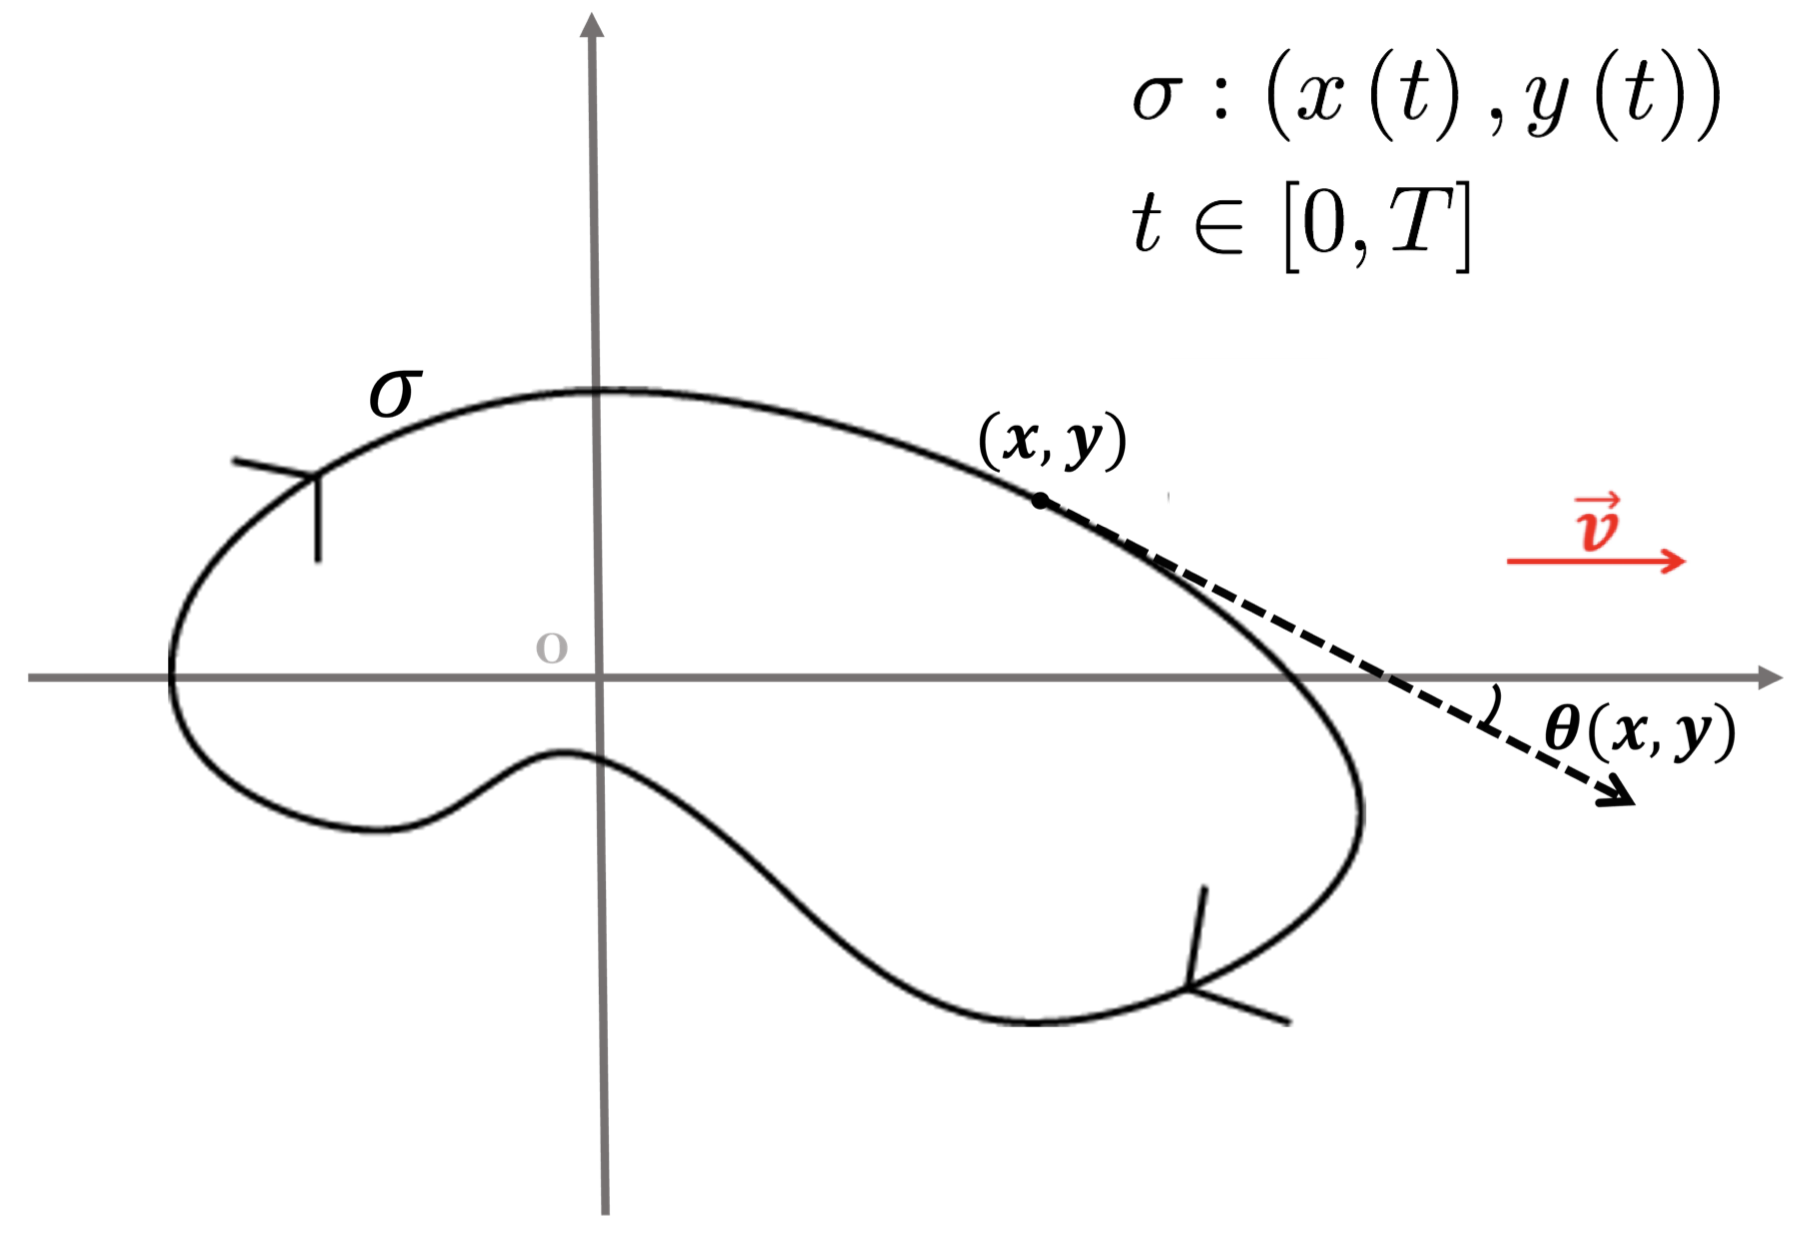
\includegraphics[width=0.7\linewidth]{image/fig3}
	\label{fig3}
\end{wrapfigure}

 \par A plane rectangular coordinate system is established with the wind direction as positive direction of the x-axis. Note that the circular track $\sigma$ is a $C^1$ (first-order continuously differentiable) closed curve in the plane with parametric equation as left.

{\bf Theorem 1 (Wind Direction Theorem) :} If $\sigma$ is a $C^1$ closed curve, then
\begin{equation}\label{WDT}
	\int_{\sigma} \overline{E}(1-kv^2\cos\theta)ds = \int_{\sigma} \overline{E} ds
\end{equation}
 where $\theta=\theta(x,y)=y'(t)/x'(t)$ denotes the angle between the tangent at $(x,y)$ and the x-axis. 
\begin{proof}[Proof:]

\begin{equation}
	\begin{aligned}
	\int_{\sigma} \overline{E}(1-k_1v^2\cos\theta)ds - \int_{\sigma} \overline{E} ds
	&= -\overline{E}k_1v^2 \int_{\sigma} \cos\theta(x,y) ds\\
	&= -\overline{E}k_1v^2 \int_0^T \frac{\sqrt{x'(t)^2+y'(t)^2}}{\sqrt{1+(\frac{y'(t)}{x'(t)})^2}} dt\\
	&= -\overline{E}k_1v^2 \int_0^T x'(t) dt\\
	&= -\overline{E}k_1v^2 (x(T)-x(0))\\
	&= 0
\end{aligned}
\end{equation}
\par For $\sigma$ is a closed curve, $x(T)=x(0)$. The variable substitution formula of the first type curve integral is used at the second equal sign.
\end{proof}
\par Wind Direction Theorem implies that the effect of wind direction on the total energy (per kilometer) required to complete the race is only relevant to the start and finish, instead of the condition of each track. The mathematical explanation is presented below:
\begin{wrapfigure}{l}{6cm} % 靠文字内容的左侧
	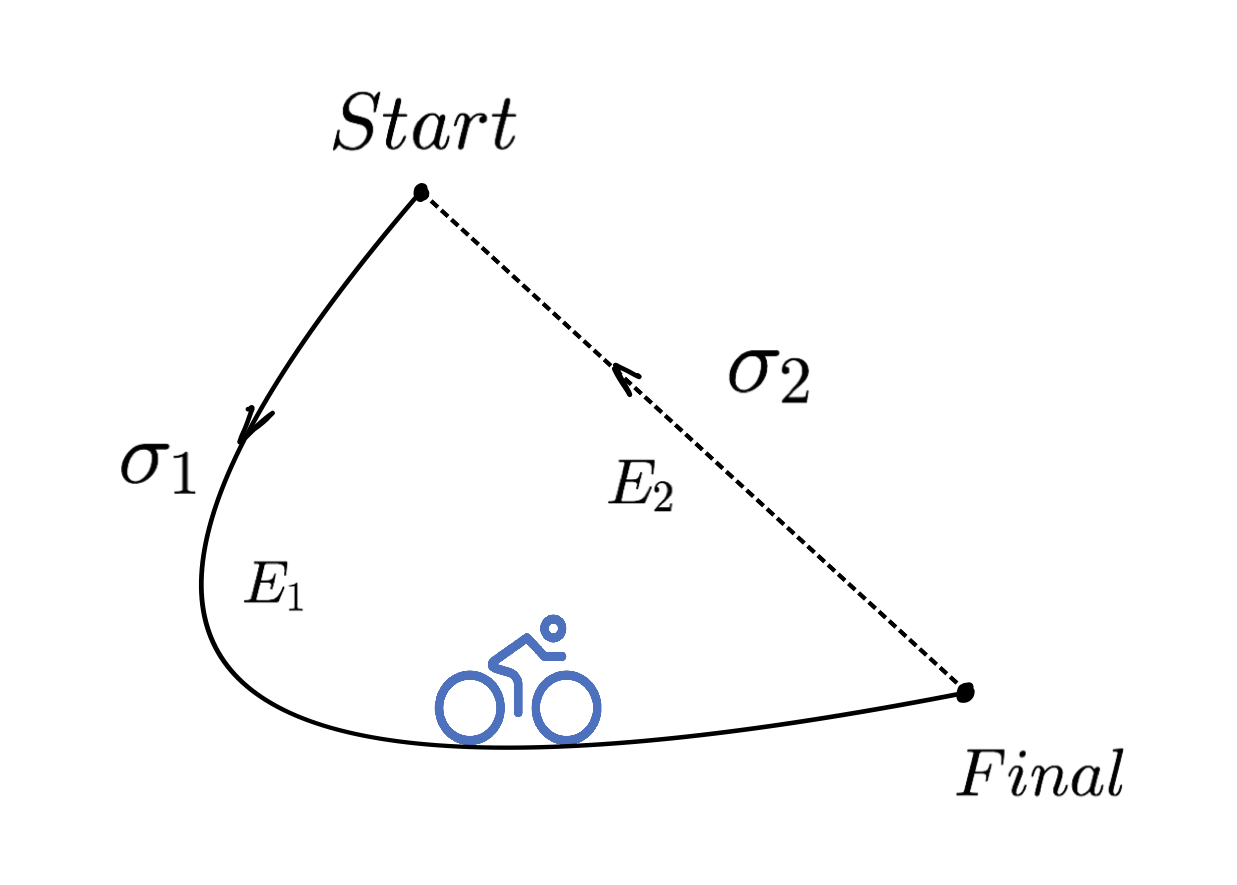
\includegraphics[width=0.9\linewidth]{image/fig1}
	\label{fig1}
\end{wrapfigure}
  \par The track is represented by $\sigma_1$, and $\sigma_2$ denotes the line connecting start and final. Let $E_i$ become the energy cost per kilometer on $\sigma_i$ while there exists wind, and $\Delta E_i=E_i-\overline{E}$. The length of $\sigma_i$ is $L_i$.

\par According to Wind Direction Theorem, it is true that
\begin{equation}
	E_1L_1+E_2L_2=\overline{E}(L_1+L_2)
\end{equation}
\par That is to say, $\Delta E_1 = \frac{\Delta E_2L_2}{L_1}$.
\par In conclusion, Wind Direction Theorem and its corollary indicate that wind direction and speed does not affect the total energy cost of a circular track. In other cases, the total cost of energy can be calculated by Start, Final and distance.
\subsection{Impact of Weather Speed}
As discussed before, increase or decrease in total energy consumption due to wind is only related to wind speed, starting and end position. So in this part, we only talk about a non -closed route: UCI World Championship time trial course in Flanders.
\par Take UCI World Championship time trial course for men as an example, it's obvious that the straight line distance between start and end points can be calculated easily, which is important to the analysis of wind effect.
\par As discussed above, $E(s)$ can be described as follows according to Eq (\ref{E}):
\begin{equation}
	E(s) = \overline{E}(1-k_1v^2\cos\theta(s))
\end{equation}
where $v$ is a constant wind speed. 
\par Using our virtual rider MTT and FTT, we can simulate the model of this track at different wind speeds and solve out the optimal strategy. Then we can get results as table [\ref{wind}][\ref{wind2}].
% Table generated by Excel2LaTeX from sheet 'Male'
\begin{table}[h]
	%	\renewcommand\arraystretch{1.3}
	\setlength\tabcolsep{13pt}%调列距
	\setlength{\belowcaptionskip}{0.2cm}
	\centering
	\caption{Minimum time for men to finish UCI WCTT under weather condition}
	\begin{tabular}{c|ccccc}
		\toprule[2pt]
		& Wind Speed & $T_1$  & $T_2$  & $T_3$  & Total \\
		\midrule
		\multirow{2}[2]{*}{Upwind} & 15 mph    & 28:51 & 7:19  & 7:14  & 43:24 \\
		& 5 mph    & 28:51 & 9:56  & 7:14  & 46:01 \\
		\midrule
		No wind & 0     & 28:51 & 12:40 & 7:14  & 48:45 \\
		\midrule
		\multirow{2}[2]{*}{Downwind} & 5 mph     & 28:51 & 15:08 & 7:14  & 51:13 \\
		& 15 mph     & 28:51 & 17:44 & 7:14  & 53:49 \\
		\bottomrule[2pt]
	\end{tabular}%
	\label{wind}%
\end{table}%

% Table generated by Excel2LaTeX from sheet 'Female'
\begin{table}[h]
%	\renewcommand\arraystretch{1.3}
	\setlength\tabcolsep{13pt}%调列距
	\setlength{\belowcaptionskip}{0.2cm}
	\centering
	\caption{Minimum time for women to finish UCI WCTT under weather condition}
	\begin{tabular}{c|ccccc}
		\toprule[2pt]
		& Wind Speed & $T_1$  & $T_2$  & $T_3$  & Total \\
		\midrule
		\multirow{2}[2]{*}{Upwind} & 15 mph    & 19:25 & 3:17  & 8:49  & 31:31 \\
		& 5 mph    & 22:22 & 3:19  & 8:49  & 34:30 \\
		\midrule
		No wind & 0     & 26:20 & 3:18  & 8:49  & 38:27 \\
		\midrule
		\multirow{2}[2]{*}{Downwind} & 5 mph     & 28:19 & 3:18  & 8:49  & 40:26 \\
		& 15 mph     & 31:17 & 3:18  & 8:49  & 43:24 \\
		\bottomrule[2pt]
	\end{tabular}%
	\label{wind2}%
\end{table}%
\par We can conclude from the table that male riders will change the duration of recovery according to weather condition, while female riders will change FTP time($T_1$).
\par In all conditions, the virtual male rider exerts his strength at the level of FTP in the first period  $T_1$, and recover for 21:16(min), controlling his average power output per weight at 6.40 W/kg. in the final sprint, he exerts all effort over the level of FTP, maintaining 7.16 power output per weight, and finally scores 57:12(min). The same goes for the analysis of women, whose power output per weight is FTP, 5.61 and 6.34 separately.

